\chapter{Evaluation}
\chaptermark{Evaluation}
This evaluation is split up into \FetchStoredCounterValue{section} sections. The first \autoref{sec:evaluation: ontology} is about our used ontology, how realistic the modelling is, and whether our implementation is comfortable.   Then, we evaluate our fragmentation strategies in \autoref{sec:frag:eval}. The important \autoref{sec:raptor:eval} is our \glsxtrshort{raptor} evaluation, and lastly, we check our server load in \autoref{sec:load}. 

\section{Ontology}
\label{sec:evaluation: ontology}
\subsection{MongoDB storage usage}
We created a merged view for our entry point. The connected entities are embedded in our scheduled stop point. This ensures we can quickly look up each station using \glsxtrshort{raptor}.

However, we also added the rest of the information to separate collections of MongoDB. This ensures we can look up information after route planning. You can get either the entity alone or an entity and all its referenced entities. They are returned as a graph and are not embedded. The code for resolving all the references in an entity can be found in \autoref{code:resolve}. An example can be found in \autoref{code:example:line}.

\begin{table}[H]
\centering
\begin{tabular}{|l|l|l|l|l|l|}
\hline
\textbf{} &
  \textbf{\begin{tabular}[c]{@{}l@{}}Number of\\  documents\end{tabular}} &
  \textbf{\begin{tabular}[c]{@{}l@{}}Avg. \\ document size\end{tabular}} &
  \textbf{\begin{tabular}[c]{@{}l@{}}Number \\ of indexes\end{tabular}} &
  \textbf{\begin{tabular}[c]{@{}l@{}}Total\\  index size\end{tabular}} &
  \textbf{\begin{tabular}[c]{@{}l@{}}Total\\ storage size\end{tabular}} \\ \hline
AutoriteitOfOperator   & 1    & 134B     & 1 & 20.48kB  & 20.48kB  \\ \hline
Dienstkalender         & 9.7K & 24.71kB  & 1 & 151kB    & 151.57MB \\ \hline
Dienstrit              & 37K  & 309B     & 1 & 831.49kB & 2.05MB   \\ \hline
Dienstritpatroon       & 37K  & 2.27kB   & 1 & 811.01kB & 10.83MB  \\ \hline
Doorkomsttijd          & 652K & 216B     & 1 & 9.22MB   & 15.26MB  \\ \hline
Lijn                   & 856  & 479B     & 1 & 28.67kB  & 73.73kB  \\ \hline
Merged                 & 2.6K & 301.22kB & 5 & 31.07MB  & 67.70MB  \\ \hline
Route                  & 856  & 4.82kB   & 1 & 28.67kB  & 733.18kB \\ \hline
Stopplaats             & 2.6K & 209B     & 1 & 7373kB   & 98.30kB  \\ \hline
StopplaatsInRitpatroon & 652K & 715B     & 2 & 17.79MB  & 45.39MB  \\ \hline
\end{tabular}
\caption{Statistics in MongoDB of our result.}
\label{tab:mongodbstatres}
\end{table}
We can see that indexing is using a lot of storage. The problem is indexes on embedded documents are necessary to speed up our creation time.
% todo add implementation in appendix
\subsection{comformity of ontology}
\subsubsection{comformity application profiles}
\glsxtrshort{oslo} has also described when a \glsxtrshort{jsonld} document conforms to an application profile \cite{noauthor_conformiteit_nodate}.

An application profile is a specification for data exchange that introduces additional constraints for applying vocabularia. These constraints could include refinement of terminology (classes and properties) consistent with the semantics from the relevant specifications with a well-defined usage as a goal;
    External terminology (classes and properties) is used for new/extra terms not found in the existing vocabulary.

To conform with the \glsxtrshort{oslo} application profile, the following constraints have to be met:
\begin{itemize}
    \item \textbf{Must} each class contains the attributes that have a cardinality of one/
    \item \textbf{Forbidden} for a class attribute with a cardinality of maximum one to have more instantiations.
    \item \textbf{Forbidden} to use terminology of vocabularia not defined in the application profile.
    \item \textbf{Allowed} to use terminology in a way that is consistent with her semantics (definition, use, domain and range)
    \item \textbf{Allowed} to extend with other vocabularies that do \textbf{do not overlap} with terminology from this vocabulary. 
\end{itemize}
\subsubsection{\glsfmtfull{shacl}}

The \glsxtrshort{oslo} organisation also provides a shacl file that describes the ontology constraints. This also includes cardinality.

We tested our merged Scheduled Stop Points. First, we took one scheduled Stop point and added our context file. We then proceeded to transform the \glsxtrshort{jsonld} document to N-Quads using @rdfjs/parser-jsonld \cite{noauthor_rdfjs-baseparser-jsonld_2024}. We then read the Shacl File and provide both turtle files to the \glsxtrshort{shacl} validator \cite{noauthor_rdf-validate-shacl_2024}. The code can be found in the appendix \autoref{code:shacl:validator}.

\begin{listing}[H]
    \inputminted[frame=single,linenos,breaklines]{JSON}{code/shacl_1.json}
    \caption{In Our first results, we wrote "tot" instead of "Dienstverbinding.tot", triggering the less than one value constraint.}
    \label{code:json:shacl}
\end{listing}


We got good results, but we found a mistake. Visible in \autoref{code:json:shacl}. The uncovered problem is that we miswrote a field of Dienstverbinding. Another primary constraint was a ClassConstraint violation. Mainly, this was caused by the fact that the entity that a \glsxtrshort{iri} was pointing to was not in the graph.

\section{Fragmentation evaluation}\label{sec:frag:eval}
We wrote a quick Python script for a first but straightforward evaluation of our fragment strategies. The duration (\autoref{fig:fragduration}) is the total duration to make a request, receive the request and do some processing from the client's viewpoint. The size (\autoref{fig:fragsize}) is the total size of a request, including headers.

For these measurements, a list of 100 stations was randomly selected out of all possible stations. For this, we used $random.choice()$. When a destination station was needed, we selected another 100 stations. Then, we made our requests to the server.

\begin{figure}[H]
    \centering
    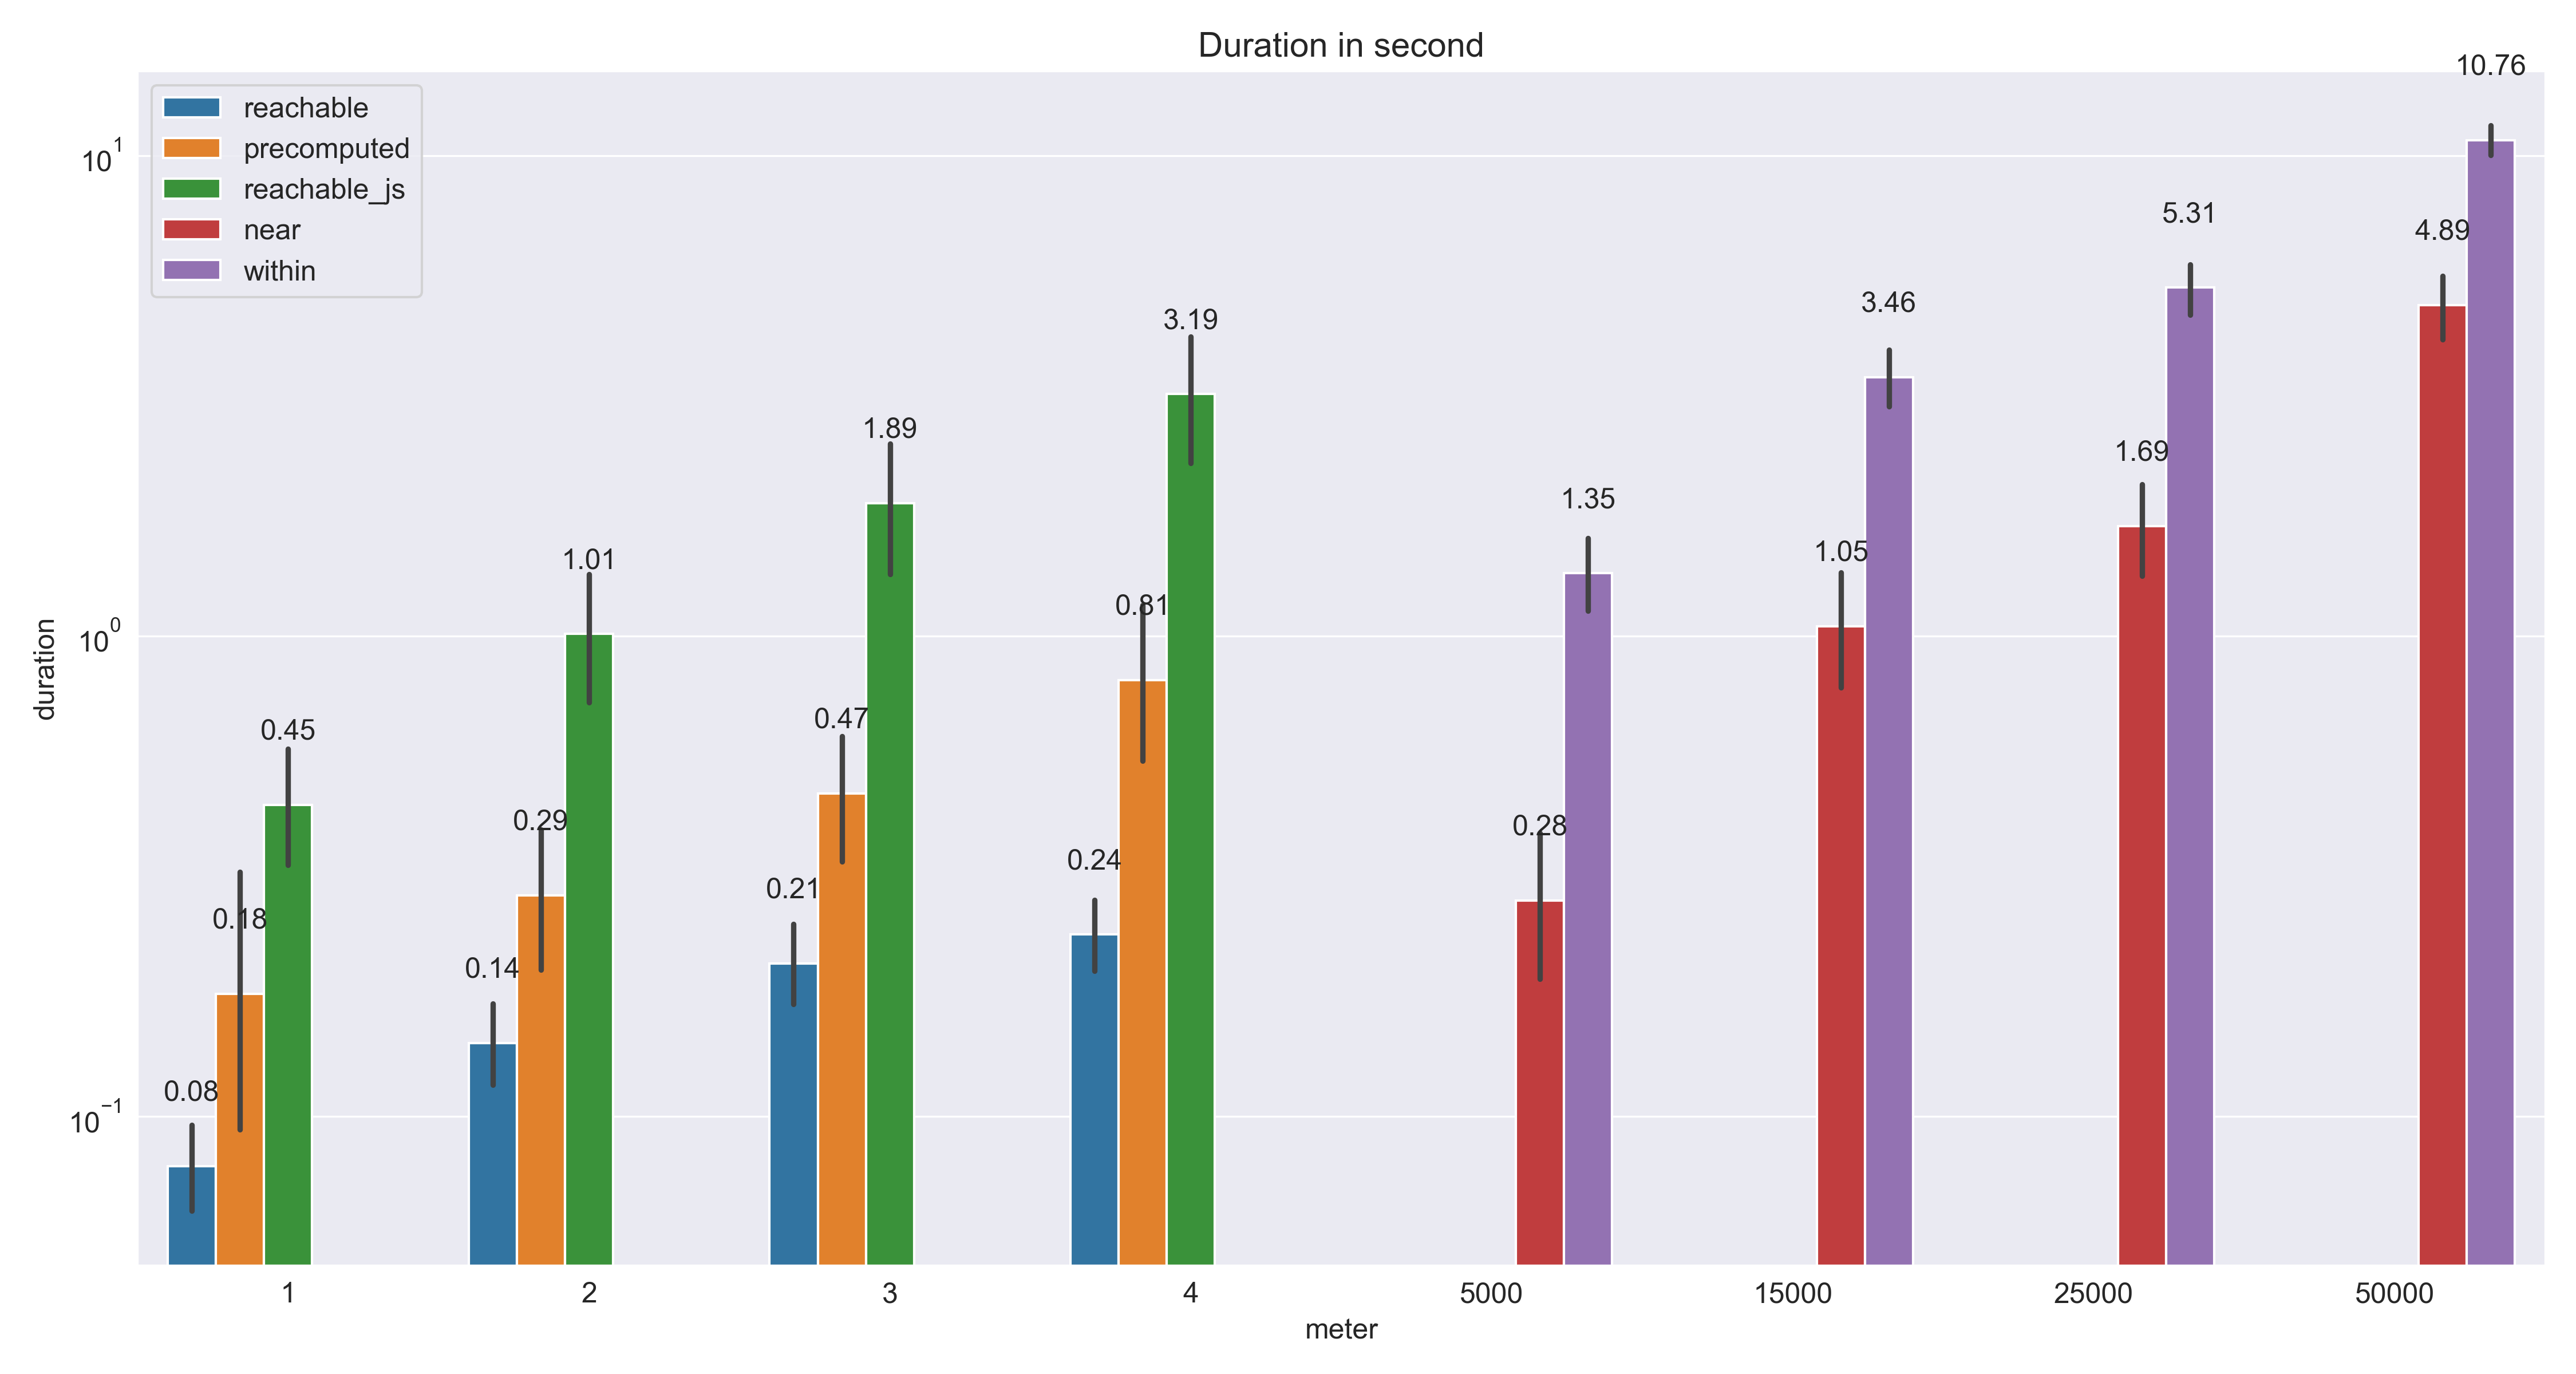
\includegraphics[width=\textwidth]{images/fragmentsbyduration.png}
    \caption{Tests measure the response and processing time needed to receive a fragment. The left four on the x-axis use a k as a parameter, and the right four use meters as a parameter. The Y-axis is in the log scale!}
    \label{fig:fragduration}
\end{figure}
\begin{figure}[H]
    \centering
    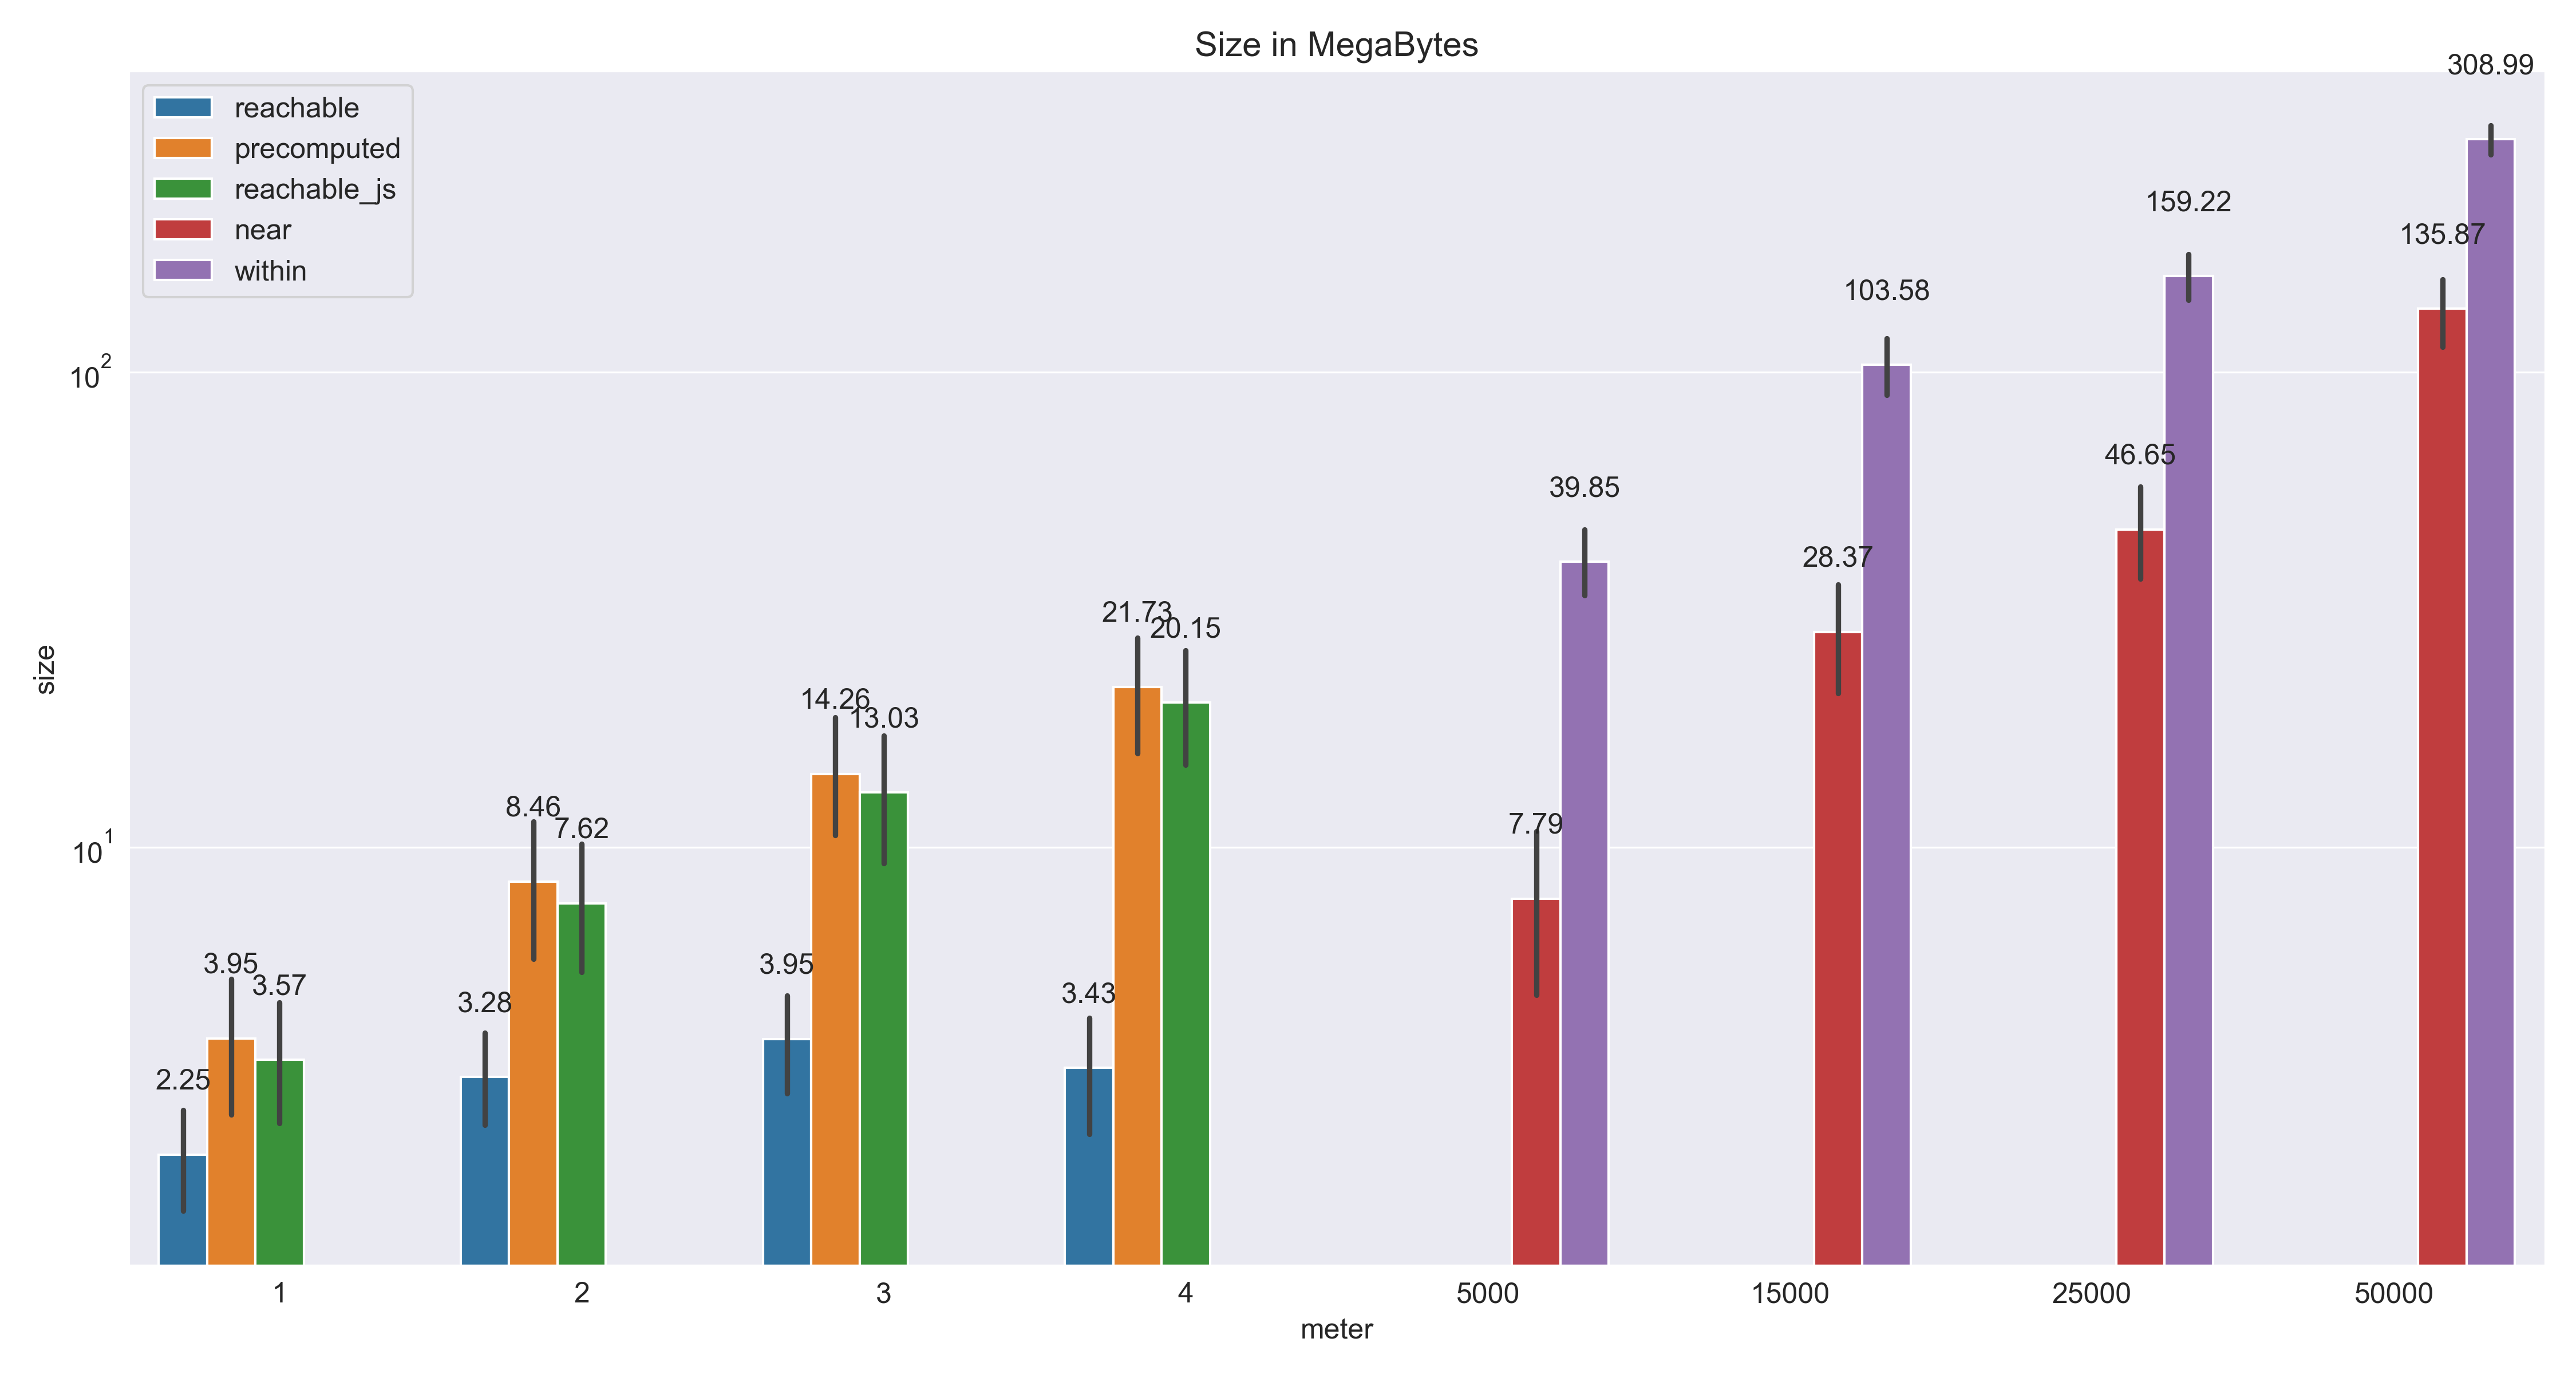
\includegraphics[width=\textwidth]{images/fragmentsbysize.png}
    \caption{Some tests to measure the size of a fragment. The left four on the x-axis use a k as a parameter, and the right four use meters as a parameter. The Y-axis is in the log scale!}
    \label{fig:fragsize}
\end{figure}


If we look at \autoref{fig:fragduration}, we see that the reachable strategy is the fastest. The JavaScript version quickly becomes slower with higher k values. The precomputed version indeed saves time compared to the javascript version. 

The reachable implementation using $\$graphLookup$ is the fastest, but we can not trust the graph as K grows. As graphlookup errors, when passing the 16 Megabyte limit, it can only handle the subset of selected stations without many connections. 

The near strategy is fast but has trouble finding relevant stations for small values. We must use a significant parameter for long-distance travel, selecting even more irrelevant stations. 

The within strategy is generally relatively slow and has the most size. This is logical since it typically spans a large area and, depending on the buffer size contains many stations. This is probably the leading cause of its slowness. This can be seen as an advantage and a weakness. It presumably includes a lot of relevant stations; since the chance is very high, we have to pass by a station between our source and destination stations. But presumably, it also contains a lot of stations we do not pass by. We still have fewer irrelevant stations than using the near strategy. 

\section{\glsfmtfull{raptor} evaluation}\label{sec:raptor:eval}
\subsection{Randomized \glsfmtshort{raptor} test}
We randomly selected an origin and destination station to test our implementation. Then ran \glsxtrshort{raptor} on it. Per the fragmentation strategy, we repeat this 50 times. It did not always find a route, as expected. Some pairs required $K=4$, meaning four trips and three transfers. 

\begin{figure}[H]
    \centering
    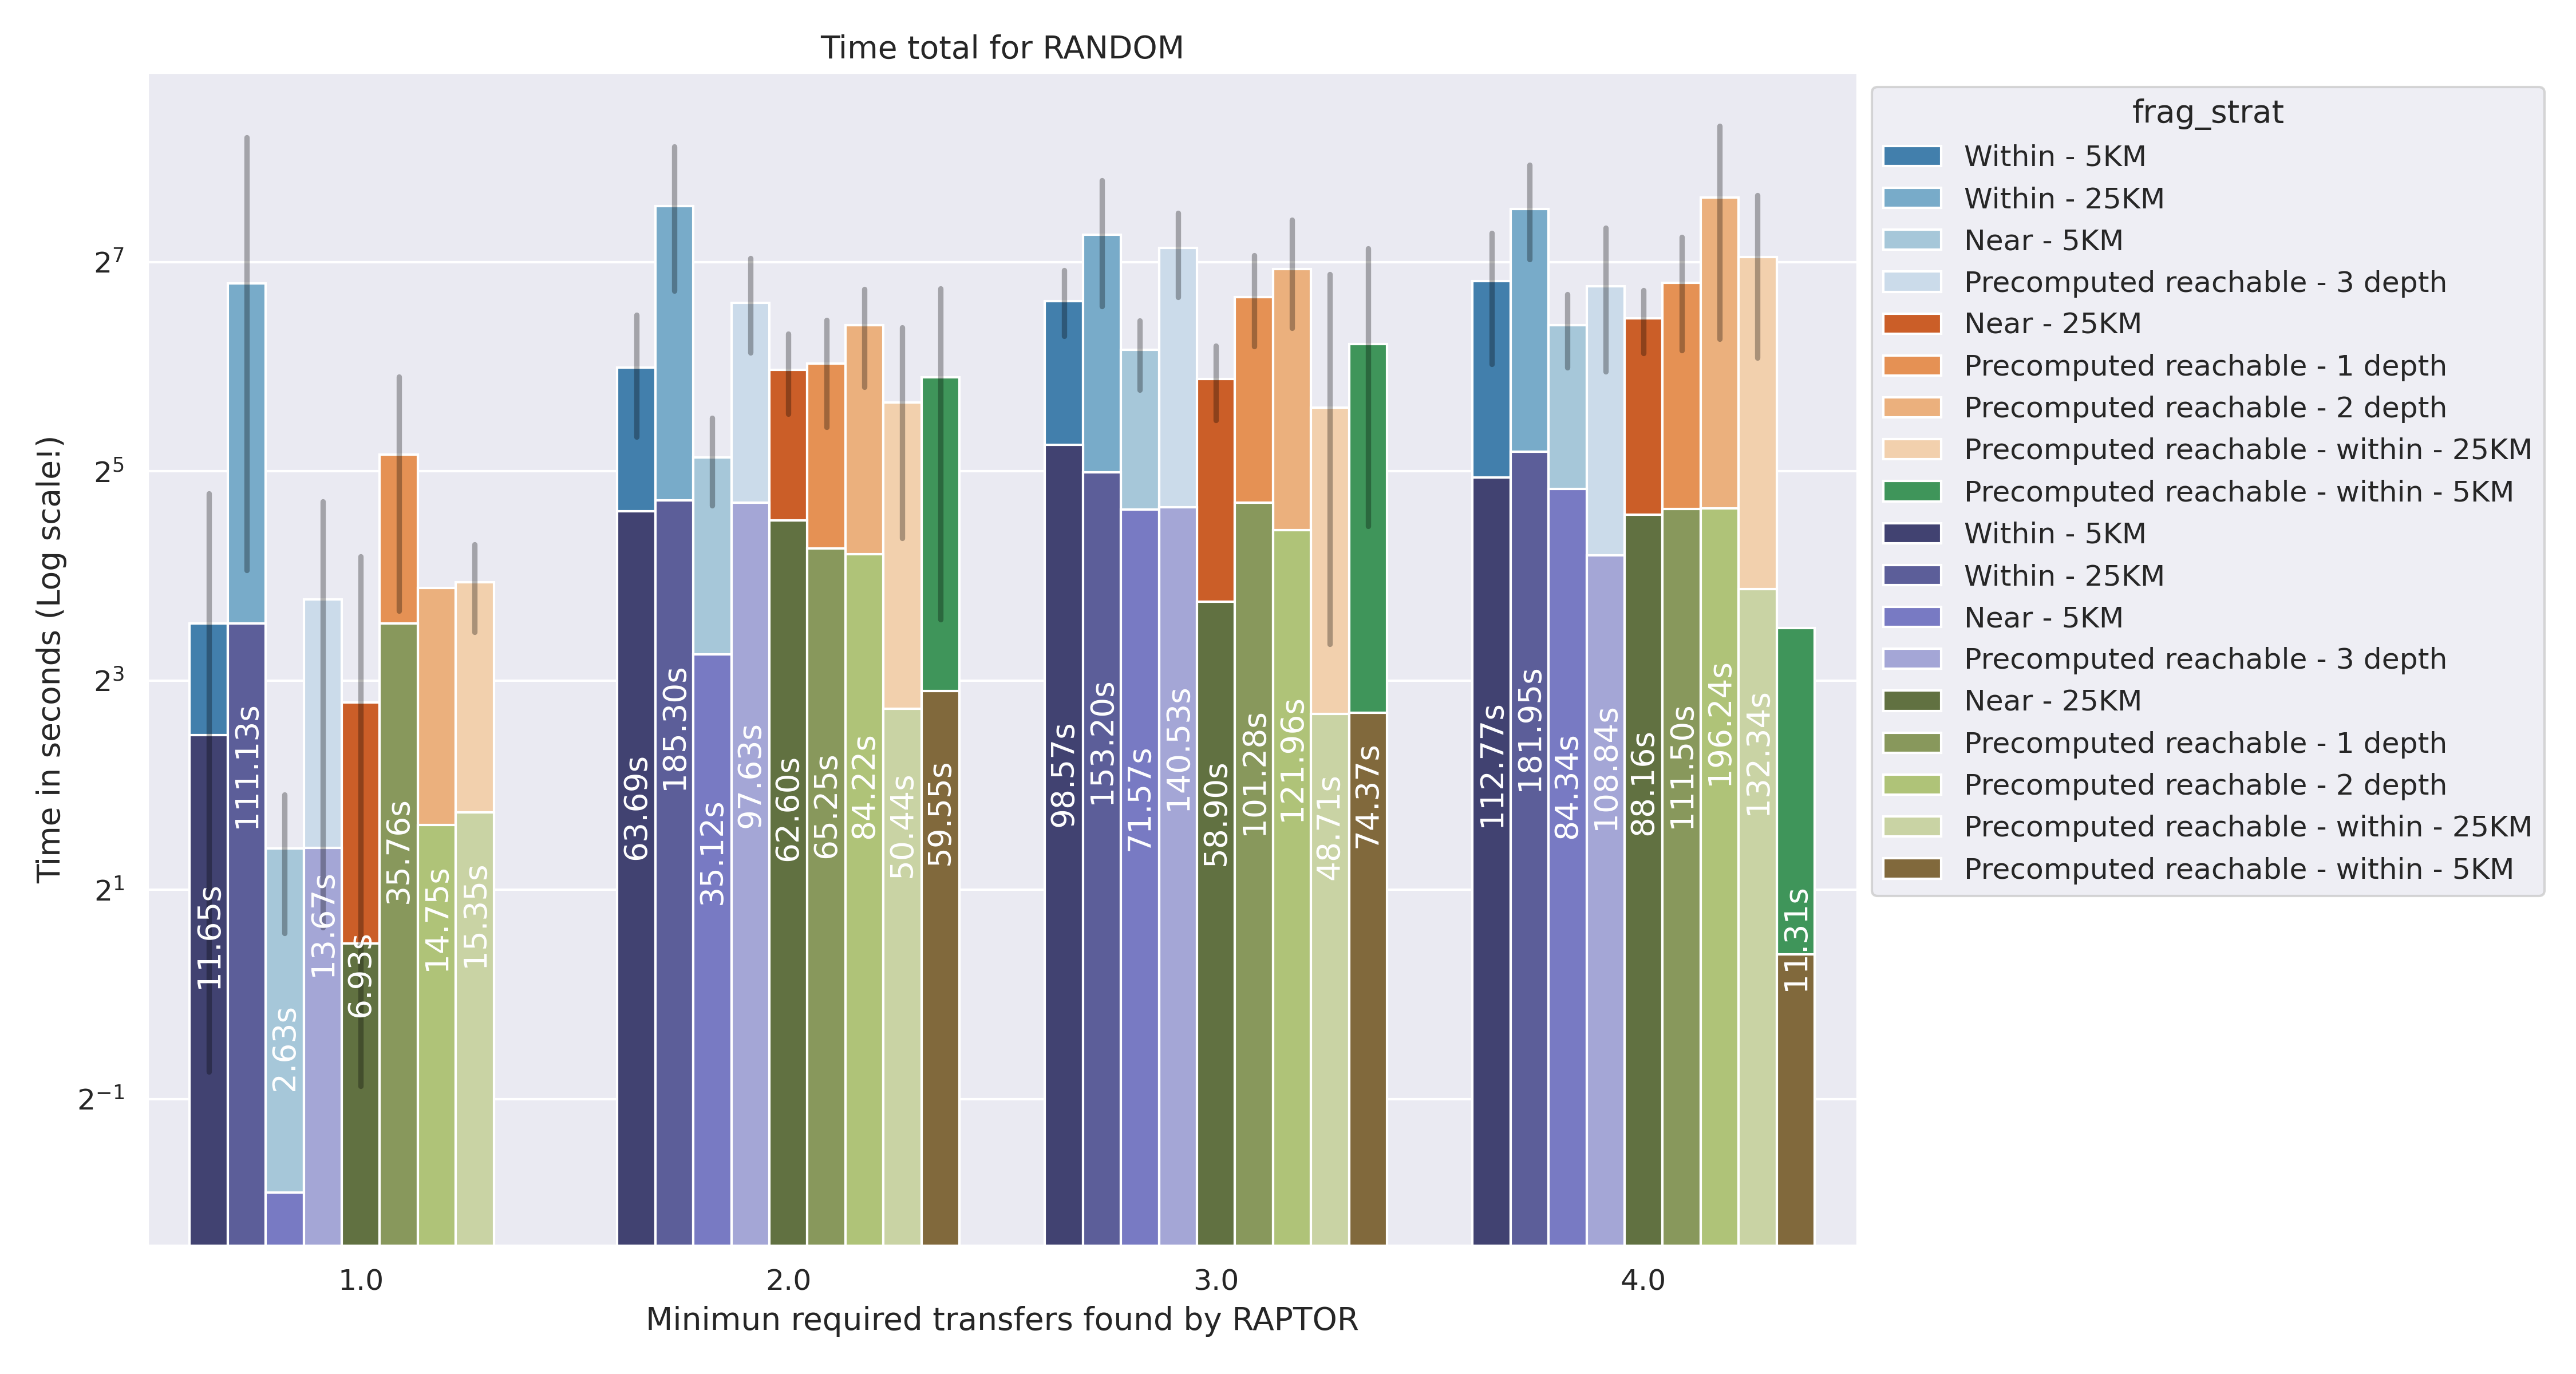
\includegraphics[width=\textwidth]{images/random_timestacked(2).png}
    \caption{Avarage time needed to solve a query. We included the total needed time and the time for \glsxtrshort{raptor} to execute. The difference between the two is due to data fetching and processing. Note that the y-axis is logarithmic. The black bars are error bars. The value in the bars is the total time.}
    \label{fig:random:timstacked}
\end{figure}

We see a sharp increase in total and raptor time between $K=1$ and $K=2$, from 12 seconds to an average of 50 seconds. This can be expected because $k=1$ are direct trips, less data has to be fetched, and Raptor does not have to look at many trips, thus less exploration. This increases substantially with $k=2$.
The difference between higher $k$ is somewhat limited, showing a less steep increase.

The geospatial strategies do not perform well due to their high response time and size. The worst performer is the Within strategy, which has a buffer of 25 km. The Reachable strategy does perform quite well. However, the combination of Within and Reachable Neighbours with a depth of three performs best.

This evaluation strategy is not the best. As random selection tends to select stations that are far away, some fragmentation strategies have no measurement in $K=1$. We have an equal problem with $k=4$ for the "Precomputed reachable—within= 5KM." There is only one measurement that resulted in $k=4$.
\subsubsection{Number of requests}
We now look at how many requests are made per strategy and the efficiency of those requests. With the number of ignored stops, we mean the stops that have been ignored because they only have been seen and processed in a previous fragment. It is an indication of an overlap.
\begin{figure}[H]
    \centering
    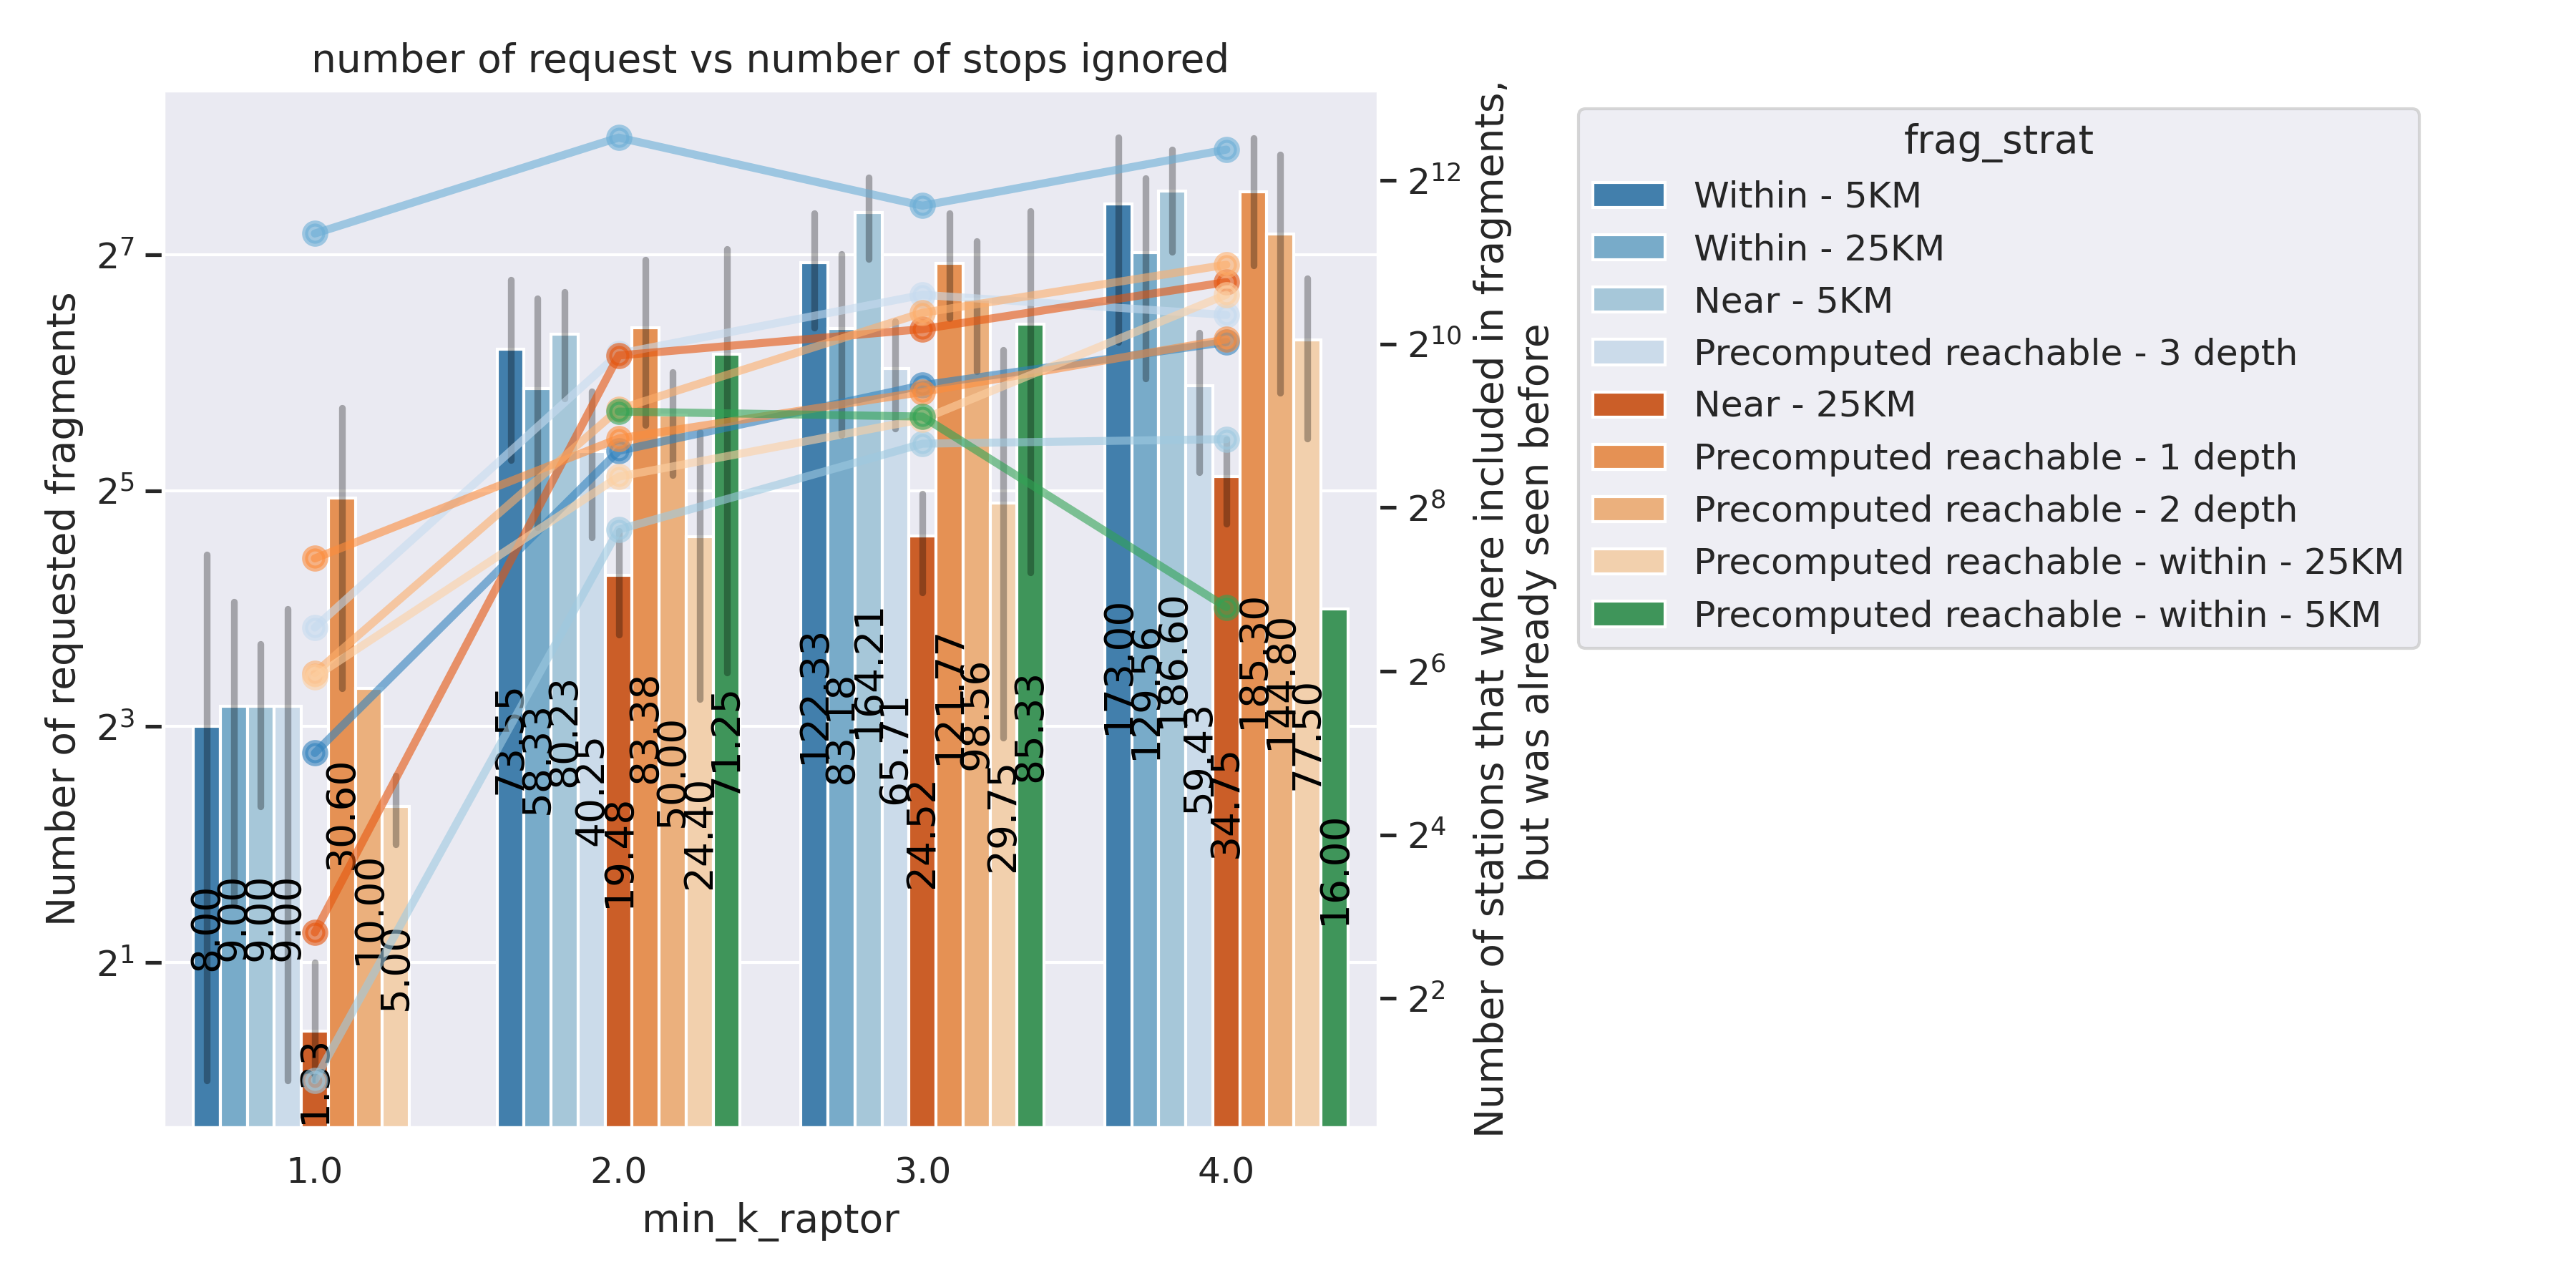
\includegraphics[width=1.1\textwidth]{images/random_request(6).png}
    \caption{Number of fragments requested per query. The lines represent the number of stops that are ignored due to overlap. Both axes are in log scale. }
    \label{fig:spentfetching}
\end{figure}

Here, we see that Within is still one of the worst performers and makes the most requests. The ignored stops are also the highest. Near 25 km makes the least requests, but for $k=2$, we see a sharp increase in ignored stops. 

When comparing reachable neighbours' strategies, a depth of one makes too many requests but decreases with depth 3. The combination of reachable neighbours and within performs well and shows a less steep "ignored stops" line.

\subsection{Curated \glsfmtshort{raptor} test}
We also tested two curated lists of routes (\autoref{app:routelist}). The first list is based on our personal travels, and the second is based on the most popular trajectories of \glsxtrshort{nmbs} \cite{noauthor_populairste_nodate}. These routes are more realistic than randomly chosen stations.

\begin{figure}[H]
    \centering
    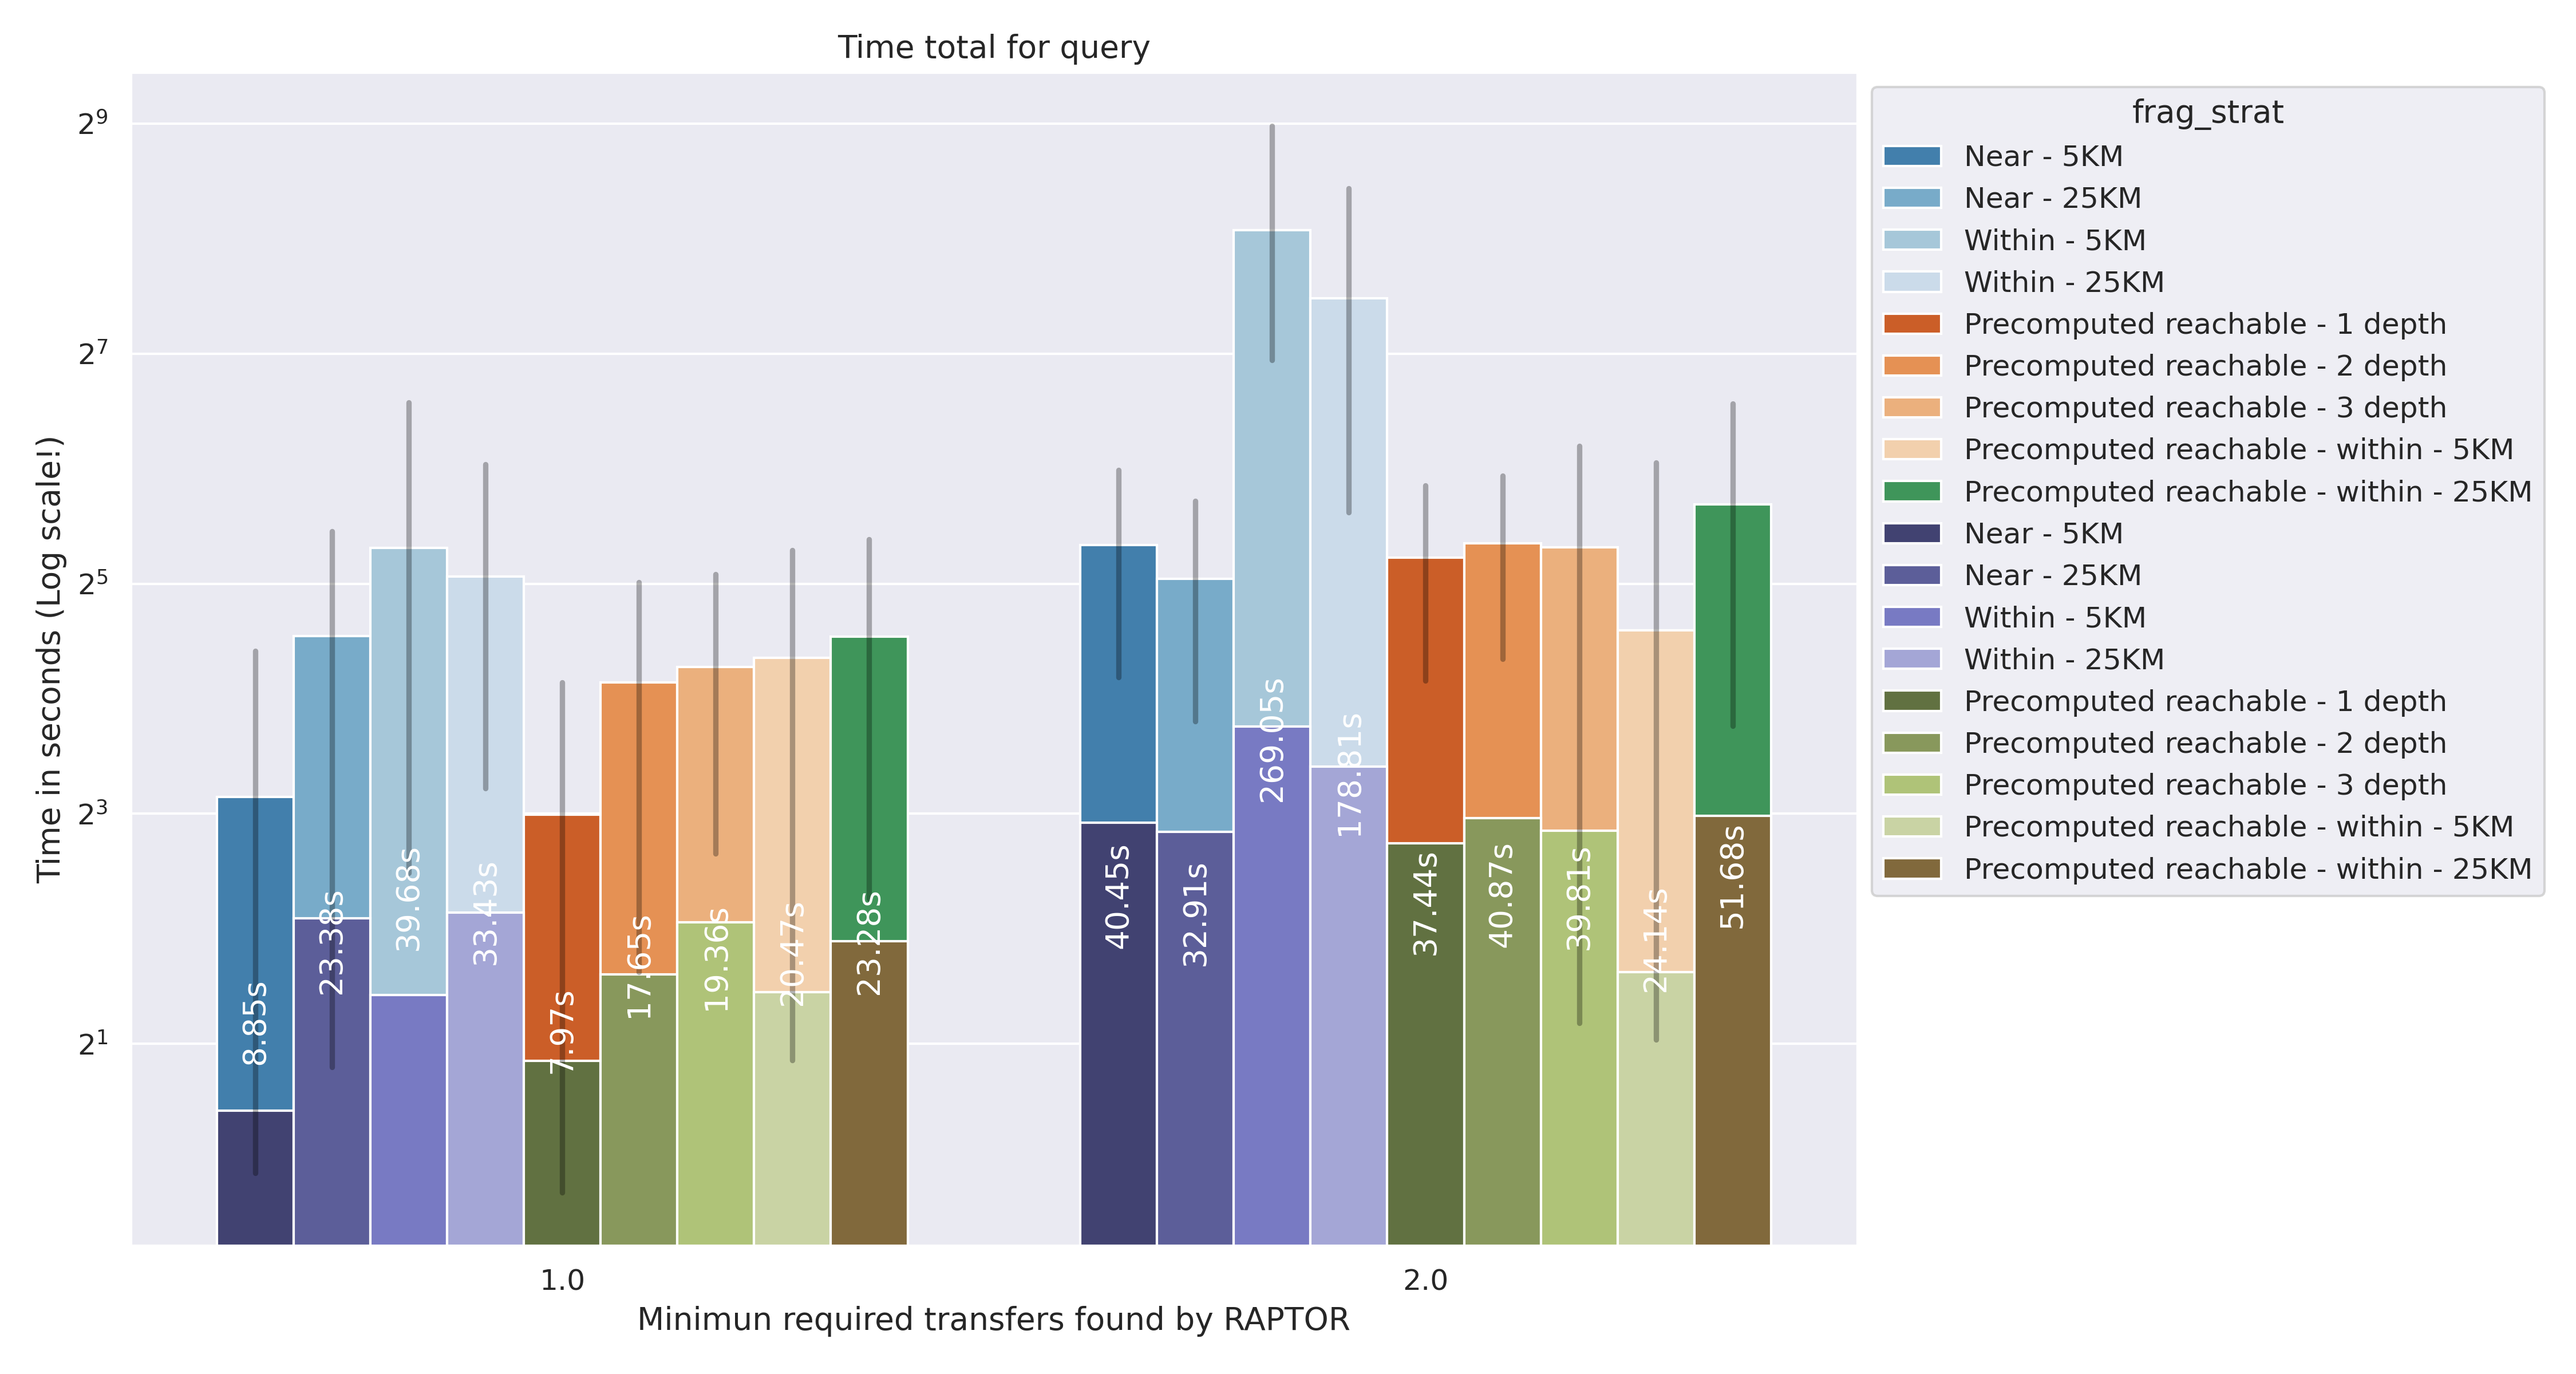
\includegraphics[width=\textwidth]{images/curated_personal_timestacked.png}
    \caption{Avarage time needed to solve a query, personally based list. We included the total needed time and the time for \glsxtrshort{raptor} to execute. The difference between the two is due to data fetching and processing. Note that the y-axis is logarithmic. The black bars are error bars. The value in the bars is the total time.}
    \label{fig:timestackedcuratedpersonal}
\end{figure}
\begin{figure}[H]
    \centering
    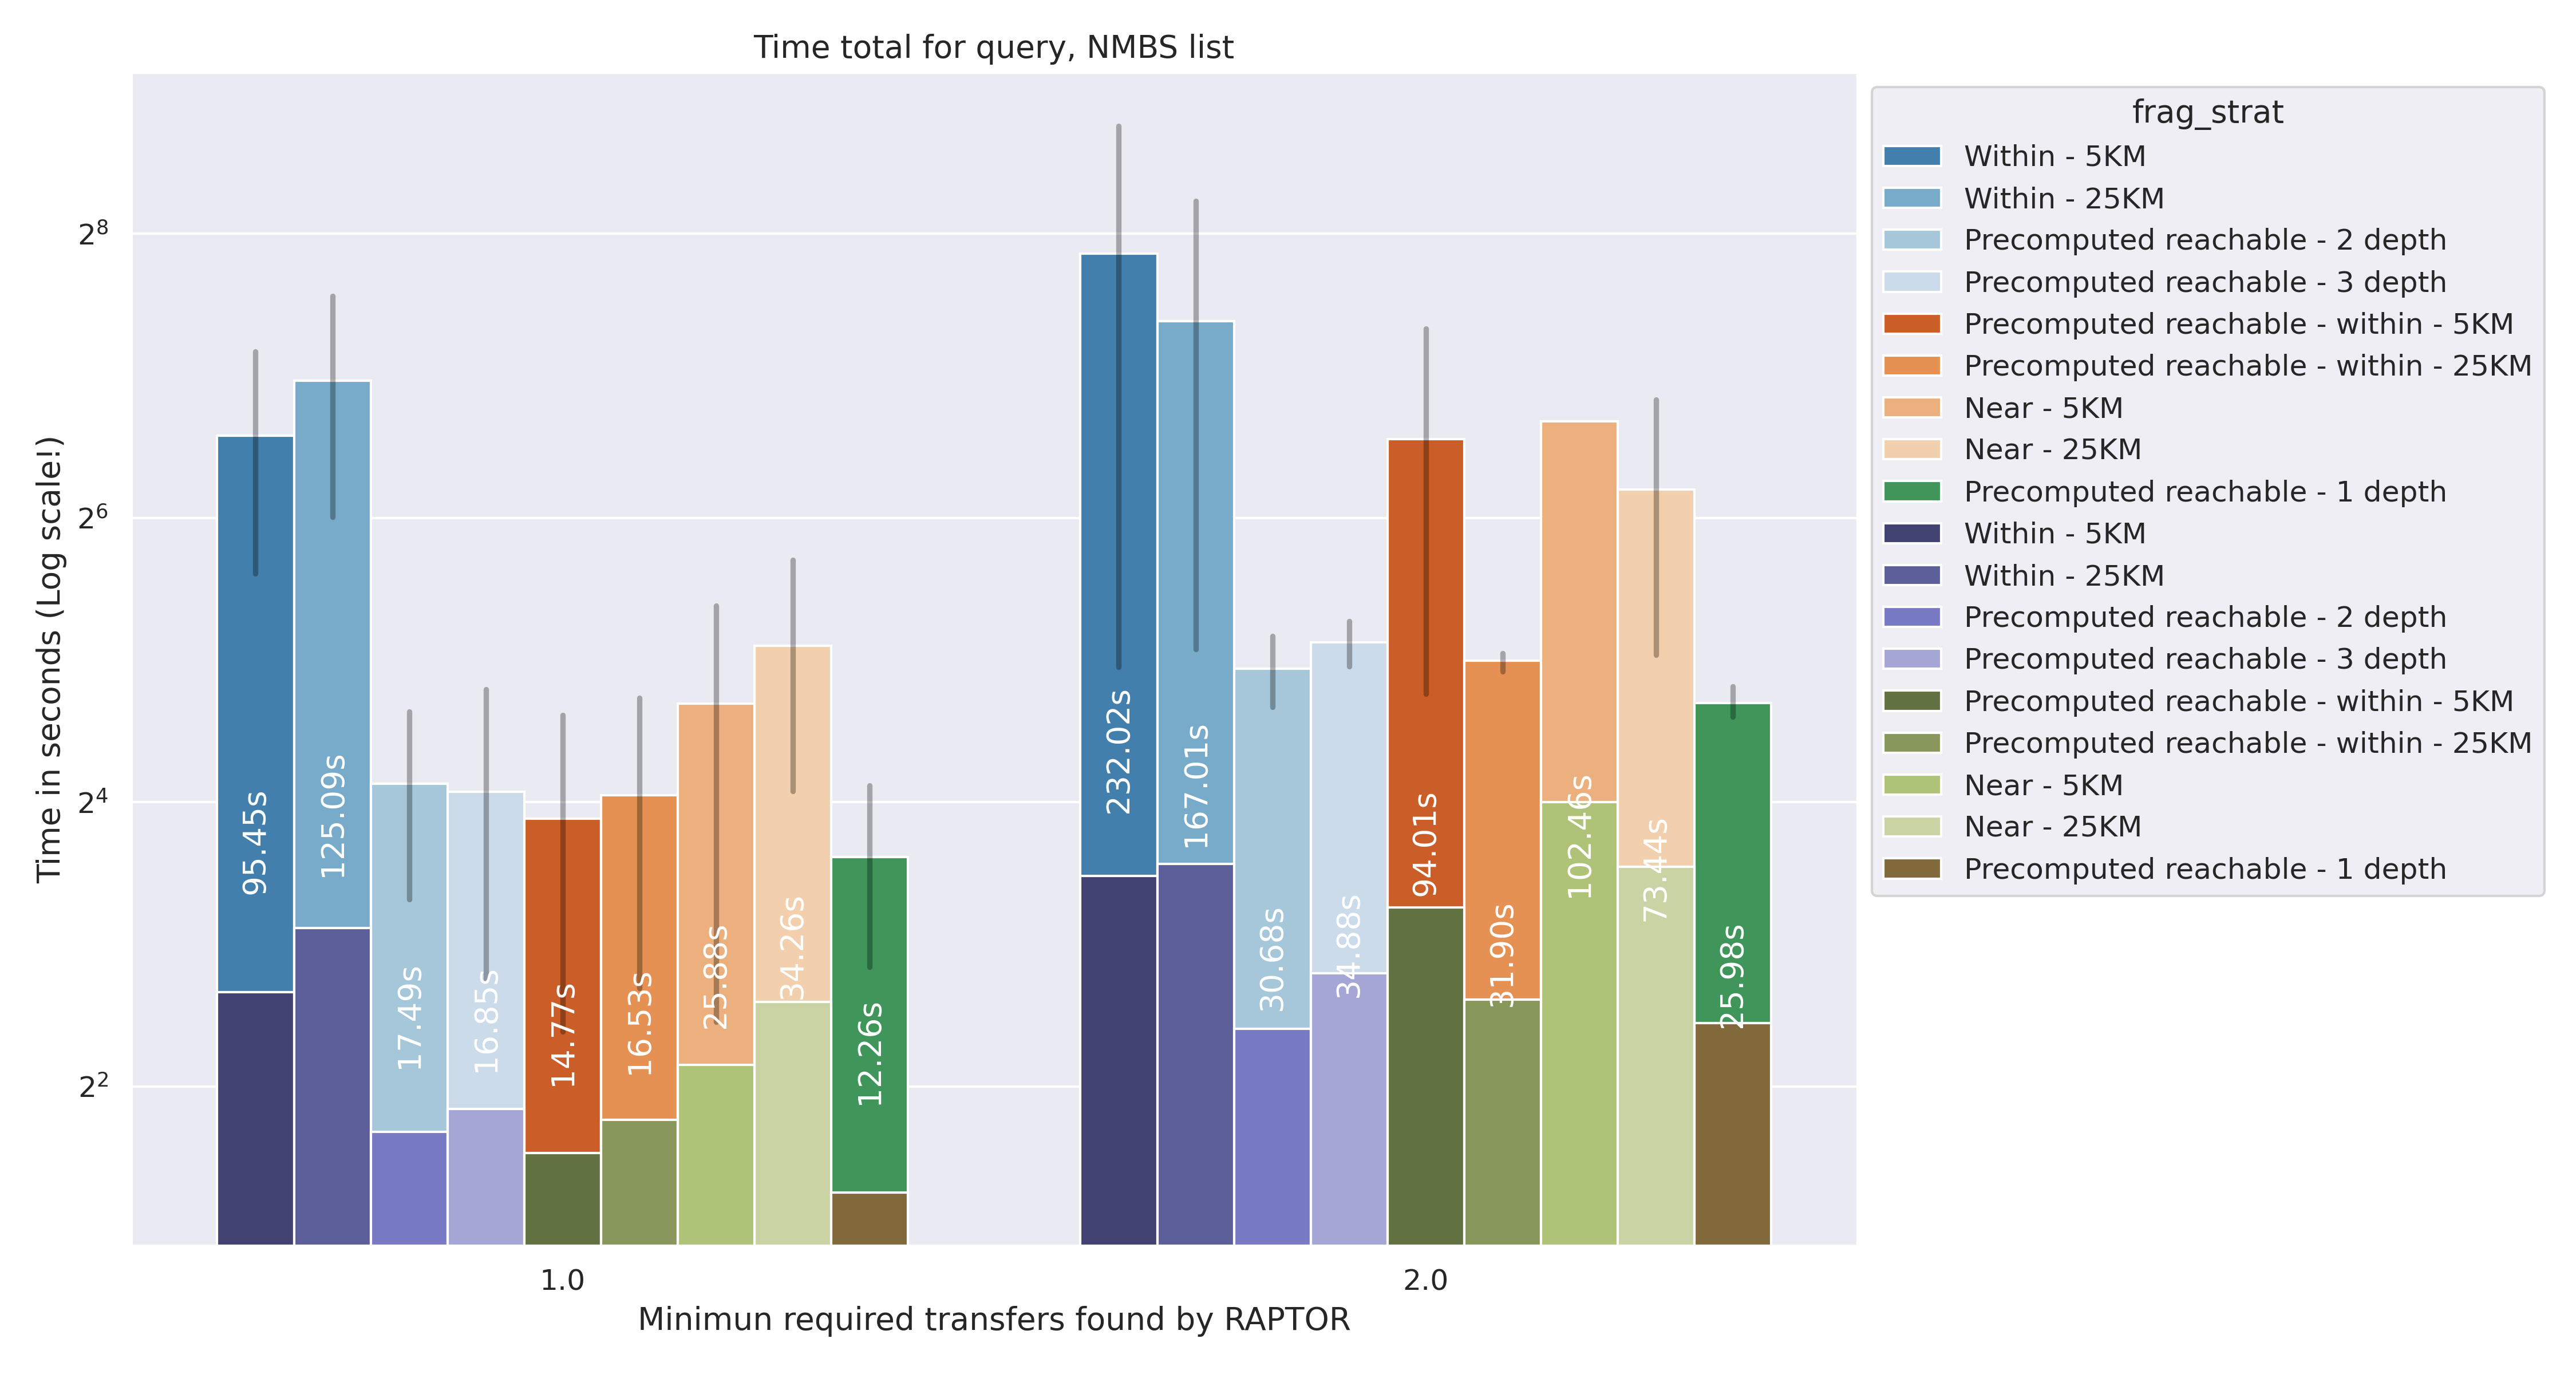
\includegraphics[width=\textwidth]{images/curated_nmbs_timestacked.png}
    \caption{Avarage time needed to solve a query, NMBS list. We included the total needed time and the time for \glsxtrshort{raptor} to execute. The difference between the two is due to data fetching and processing. Note that the y-axis is logarithmic. The black bars are error bars. The value in the bars is the total time.}
    \label{fig:curatednmbs}
\end{figure}
The averages for the personally based list (\autoref{fig:timestackedcuratedpersonal}) are lower for $k=2$; queries are taken now 40 seconds on average.

The conclusion is similar to the random evaluation. Within is the worst performer for $K=1$ and $k=2$ for both lists. 
Near does perform quite well for $k=1$ but quickly worsens for higher $k$. 

For higher $k$, reachable neighbours in combination with within is one of the better performers.
\subsubsection{Number of requests}
\begin{figure}[H]
    \centering
    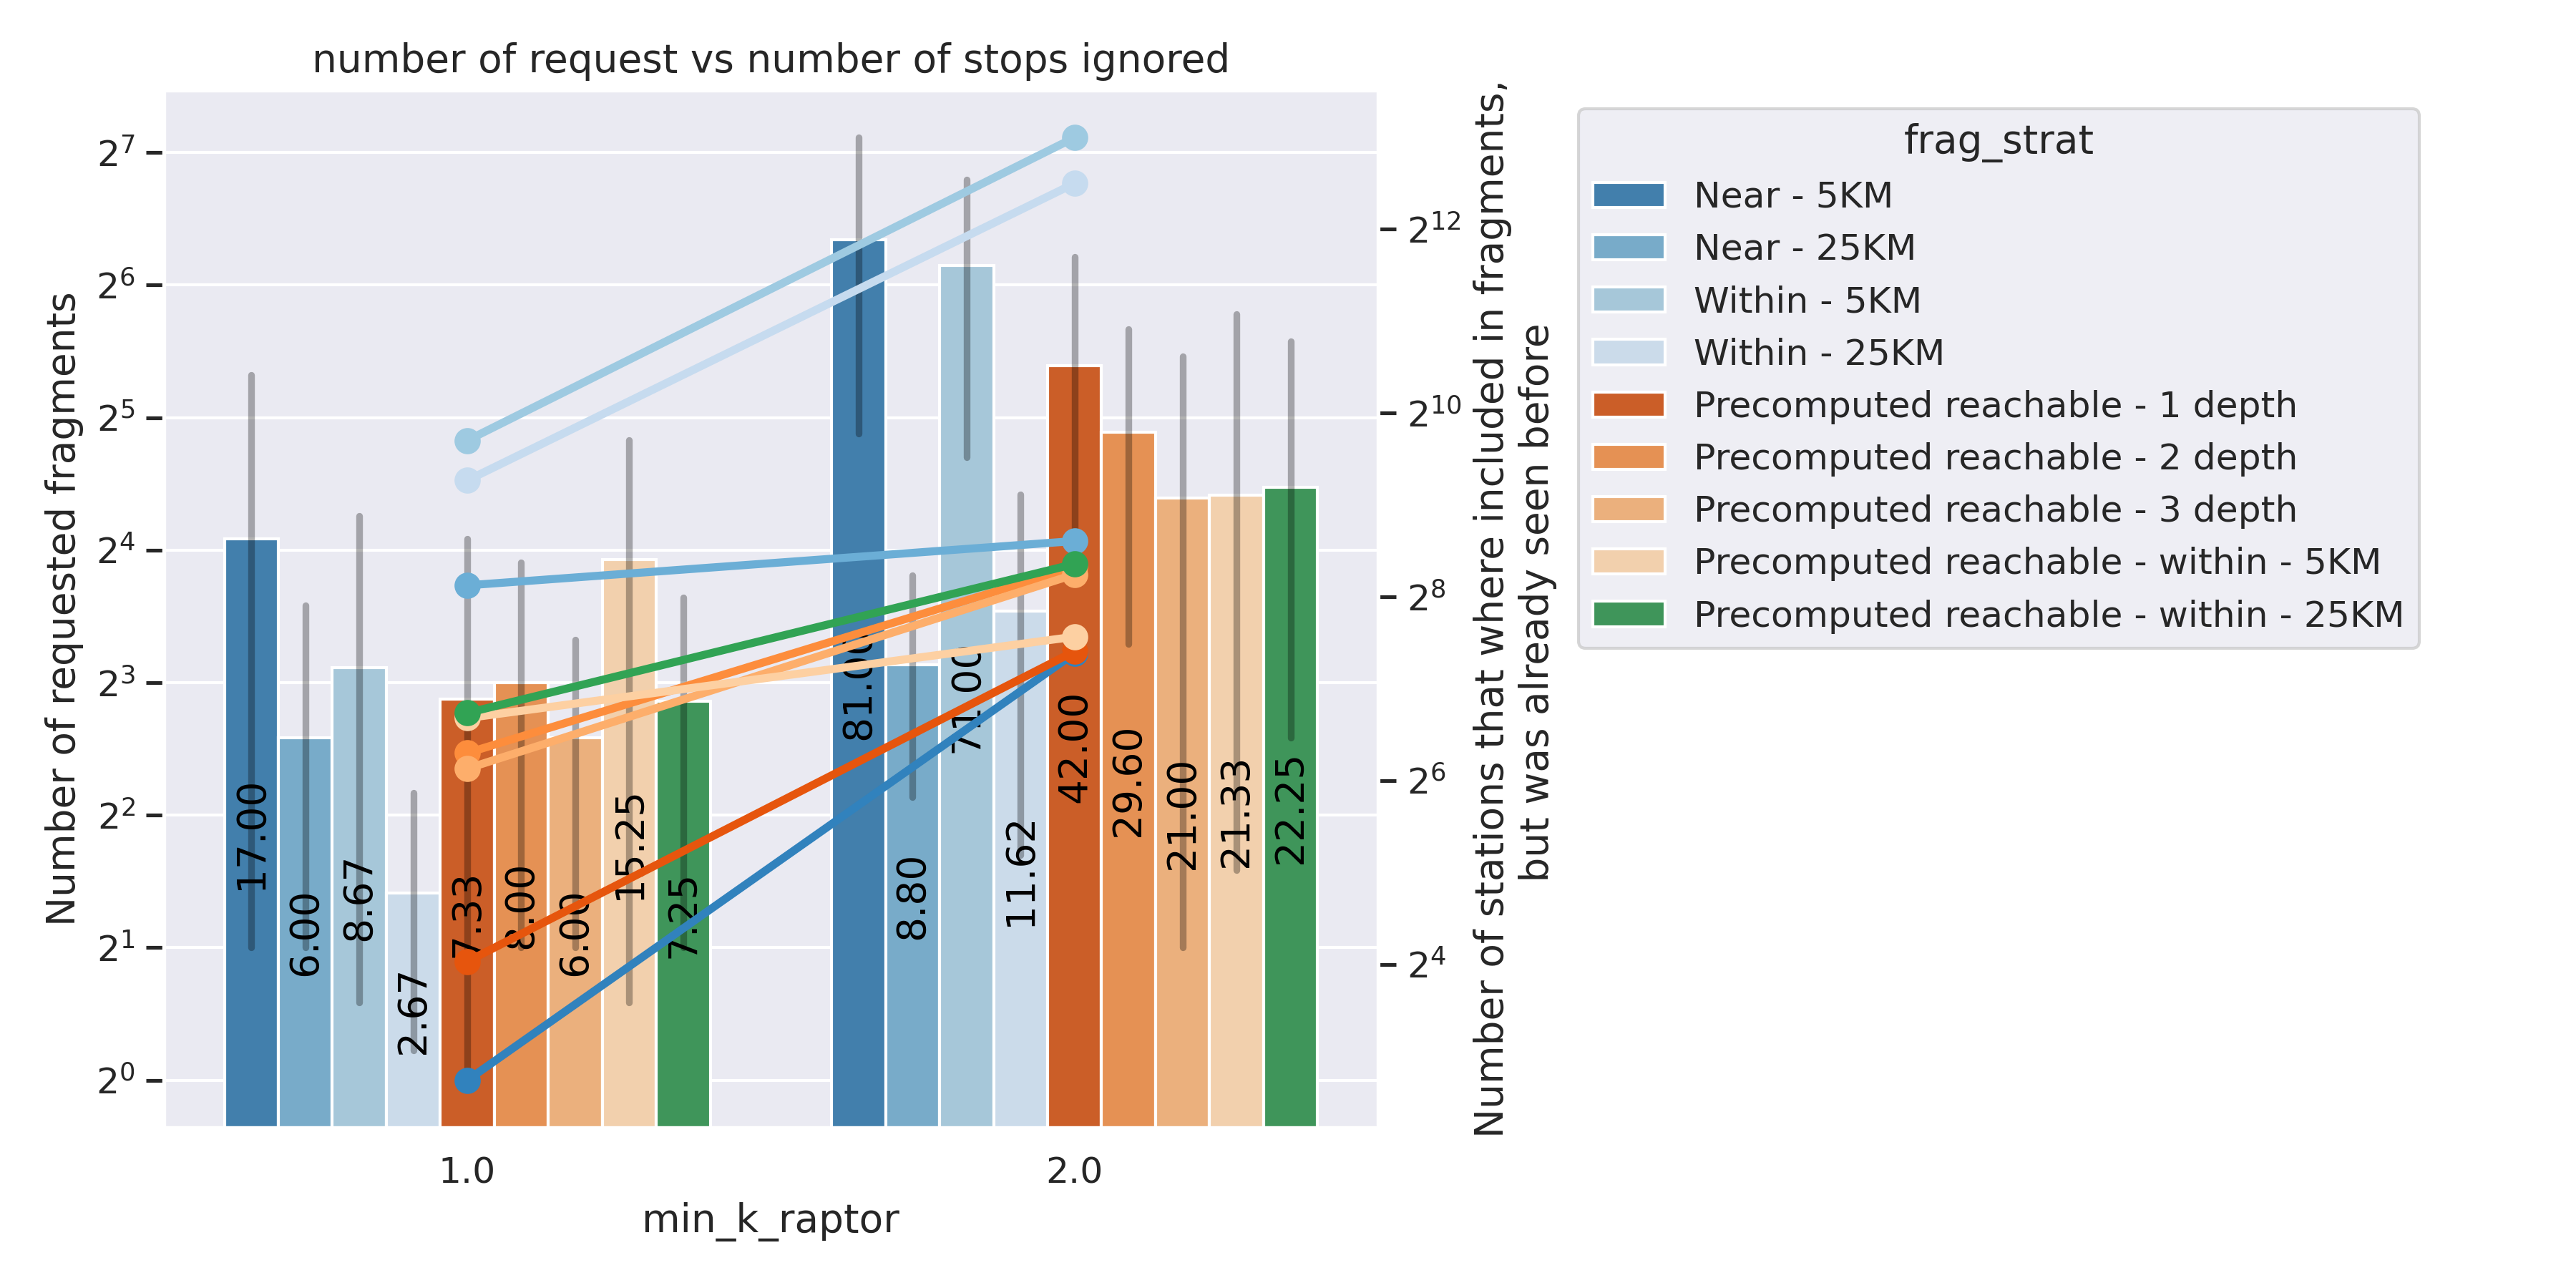
\includegraphics[width=1.1\textwidth]{images/personal_request.png}
    \caption{Number of fragments requested per query for personally based list. The lines represent the number of stops that are ignored due to overlap. Both axes are in log scale. }
    \label{fig:personalrequests}
\end{figure}
\begin{figure}[H]
    \centering
    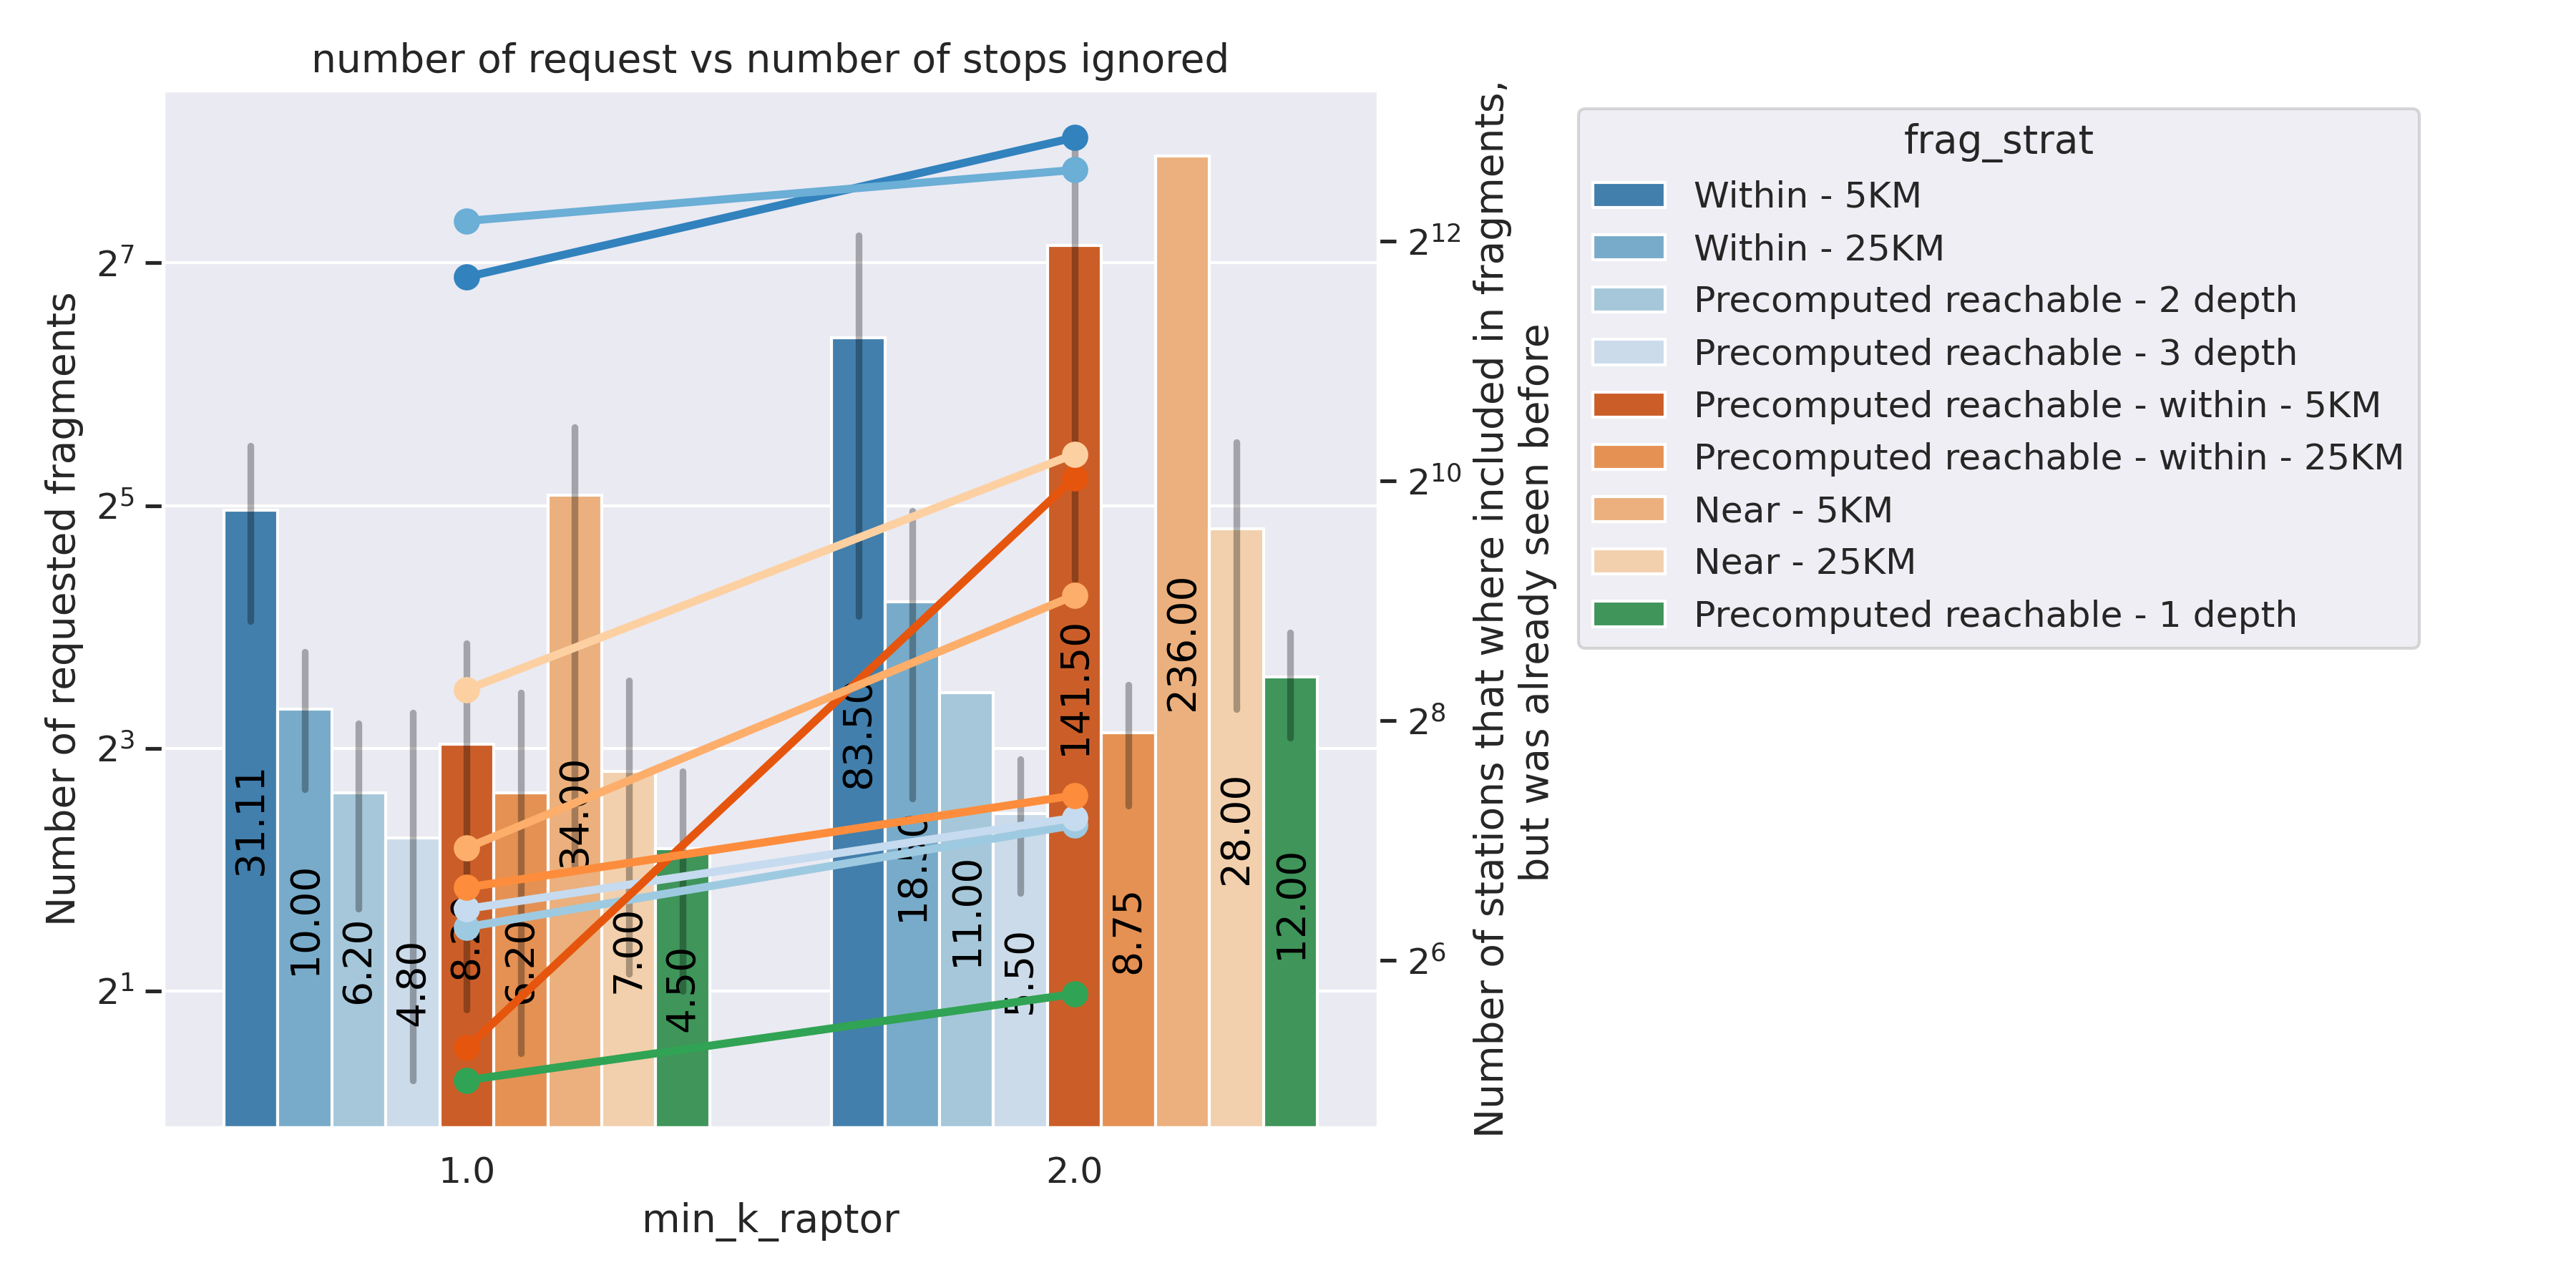
\includegraphics[width=1.1\textwidth]{images/nnmb_request.png}
    \caption{Number of fragments requested per query for the NMBS list. The lines represent the number of stops that are ignored due to overlap. Both axes are in log scale. }
    \label{fig:nmbsrequests}
\end{figure}
Globally, the same trends of the random graph (\autoref{fig:spentfetching}) are also observed in \autoref{fig:personalrequests} and \autoref{fig:nmbsrequests}. All precomputed reachable, except depth one, show a shallow line. However, the Near strategy makes more requests, and the Within strategy makes fewer requests.

Surprisingly, in \autoref{fig:nmbsrequests}, we see that Within shows a less steep incline when comparing the ignored stops of $k=1$ and $k=2$ despite making almost double the requests. The precomputed reachable within with a buffer of 5 km shows a very steep incline, which is to be expected with nearly eight times more requests.

Both figures show that reachable with a depth of three makes the least requests.
\section{Server load}
\label{sec:load}
We used the express-status-monitor \cite{noauthor_express-status-monitor_2022} to watch RAM, CPU, requests per second and heap memory. An example of such an output graph is in the appendix \autoref{fig:load}. 
Under idles, the server uses 60 MB of memory. We observe a baseline of 200-300 Megabytes of RAM under the load of 1 request per second. However, depending on the chosen fragmentation strategy, it will have very high peaks. The Within strategy, with a buffer of 25, is incredibly demanding for RAM. An upside is that the memory is quickly released when the request is handled. 

